% sections/06_method.tex — Section 6, EurekaZero: Learning Taste
% Reader question: How does a model learn taste?
% Core points advanced: 3 (search = 1) and 4 (learning from referee feedback); supports 1.
% Historical reference specifications come from the supplied source notes.
% Checkpoint acceptance and reference runtime receipts remain required.
% Historical source notes are archived outside the paper tree.
\section{EurekaZero: Learning Taste}\label{sec:method}

The reference architecture for tabular regression pairs a program writer
with a separate ranking map. Verified search supplies their training
targets; the proposed deployment protocol asks for one new program.
We describe that reference first, then distinguish the later
adapter-ranking record in \cref{sec:method-status}.

\subsection{The player in one picture}\label{sub:method-picture}

\Cref{fig:network} connects training to the single-candidate contract in
\cref{box:searchone}. A frozen encoder reads the board and the program
writer $\writer$ writes one complete program, as AlphaGo's policy
network proposed a move \citep{silver2016mastering}. The problem--program map
$\mapv$ supplies a separate ranking score. In the native implementation it
neither conditions nor screens the writer. The proposed game-day protocol
omits it, permitting only the writer's single draw under \searchone{}.

\begin{figure*}[t]
  \centering
  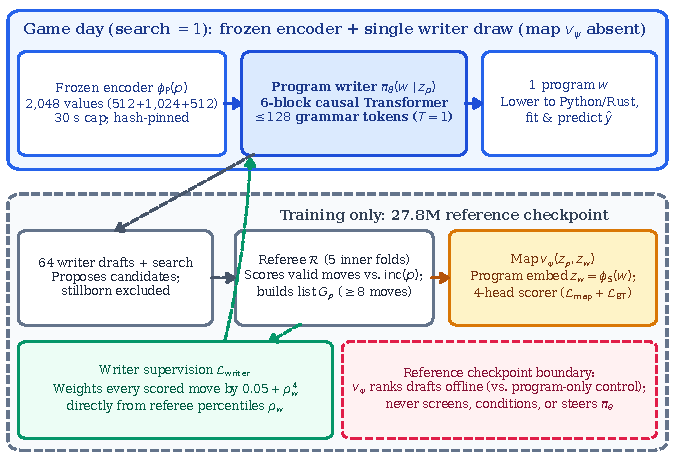
\includegraphics[width=\textwidth]{figures/fig5_network.pdf}
  \caption{\textbf{A writer and a separate ranking map learn from scored programs.} Historical reference schematic. Top:
  game day, the whole of \searchone{}. Dashed box: training only. Search seeded with the writer's
  drafts proposes more programs, the referee scores them against the incumbent, and the scored
  lists retrain the writer ($\theta$) and the map ($\psi$). Stillborn programs enter no list.}
  \label{fig:network}
\end{figure*}

\subsection{Reading the board}\label{sub:method-board}

The reference regression encoder turns the board of \cref{sec:game}
into 2,048 numbers, $z_p=\encP(p)$, in three blocks.
The first summarizes a pretrained row encoder's embeddings across rows,
independent of row order (512 values). The second projects the hidden
state of a pretrained third-party tabular regressor that reads the training
rows and labels (1,024; third-party provenance pending; restricted; redistribution prohibited). The third passes the
scaled targets through two frozen windows (512).

The reference encoder is pinned by hash and stays fixed during writer
training. Encoding is bounded at 30 seconds per problem. A context with any non-finite value is refused
rather than imputed (\cref{app:training}). The input contract permits
training-side task evidence only; final held-out labels and their derived
statistics must stay outside the input closure. A context's recorded
declaration that no final target was used establishes neither input closure
nor numerical qualification. CPU contexts require native replay and bounded-execution receipts before accepted-policy use.

Whether problems with similar best programs sit together requires a
separate representation study; \cref{sub:results-ablation} reserves that test.

\subsection{Describing the move}\label{sub:method-move}

A move is one program in the typed language of \cref{sec:game}, with a
401-token training inventory listing 31 transforms and 22 prediction heads; the product runtime restricts executable heads.
The writer emits a flat operator-and-slot token stream with a fixed
beginning, engine and regression-task header, rather than parenthesis
tokens or the \texttt{pipe} wrapper. Its nine-phase grammar mask permits
up to six transform stages and three expression stages; each expression
tree is bounded at depth four and 15 nodes
\citep{kusner2017grammar,dai2018sdvae}. After the end token, detokenization
renders a parenthesized program that must parse before entering the pool.
The mask has no remaining-token-budget check: a draw without an end token
at the 128-token horizon, including the fixed header, is incomplete and
discarded. Grammar legality does not establish successful execution or
useful quality. The proposal
pool removes exact decoded-string duplicates and records their SHA-256.
The executor also records canonical recipe hashes. Probe-based behavior
matching is a separate audit, not part of pool deduplication. Without probe
evidence, this behavior check reports novelty as unknown. Readable Python
and Rust exports are a reference requirement. Legacy recipe emitters reject
the synthesized input stage; the separate fitted-state path is allowlisted.
Reported winners still require the parity check in \cref{sub:method-referee}.

\subsection{One map for problems and programs}\label{sub:method-map}

The map reads a program as $z_w=\encS(w)$, the layer-normalized mean of
non-padding token embeddings, including \texttt{BOS}, the fixed engine and
task header, and \texttt{EOS}. Pooling discards token order, limiting its
ability to distinguish compositions built from the same tokens.

The map's own two-layer context network projects the 2,048-value $z_p$
to $r_z\in\mathbb{R}^{512}$. It joins three 512-value blocks: $z_w$
as is, $z_w\odot\tanh(W_\gamma r_z+b_\gamma)$, and
$|z_w-(W_{\mathrm{proj}}r_z+b_{\mathrm{proj}})|$.
Four two-layer heads receive this same 1,536-value interaction vector;
their mean gives $\mapv(z_p,z_w)$ with parameters $\psi$.
Native ranking losses supervise that mean jointly, without separate
targets or bootstrap samples. Training applies dropout of 0.05 in each
ranking head. The runtime head instead reads $[r_z,z_w]$, while the
program-only control reads $z_w$.

Higher logits rank higher within a problem. The score is not a calibrated
error estimate. Comparing its magnitude across problems or reading it as a
probability of a verified win requires separate evidence. The referee
still establishes validity and measures performance.

The map learns from scored lists. For each problem $p$ with at least eight
scored programs, $G_p$ holds them and $\rho_w\in[0,1]$ is a program's
percentile, 1 for the best. The map's softmax over the list is trained toward a target concentrated on the best
\citep{cao2007listnet}:
\begin{equation}
  \mathcal{L}_{\text{map}}(p)=-\sum_{w\in G_p}
  \frac{e^{\rho_w/\tau}}{\sum_{u\in G_p}e^{\rho_u/\tau}}\,
  \log\frac{e^{\mapv(z_p,z_w)}}{\sum_{u\in G_p}e^{\mapv(z_p,z_u)}},
  \label{eq:mapLoss}
\end{equation}
with $\tau=0.25$. With a unique best program, the low-temperature limit
concentrates the target on that program. This is a listwise ranking
objective over programs scored on the same problem; the analogy to
contrastive learning \citep{oord2018cpc,radford2021clip} does not establish
CLIP-style alignment across problems and programs.
A Bradley--Terry term adds pairwise comparisons on the same lists
\citep{bradley1952rank}. Stillborn moves have no score, so this ranking
objective covers only programs that run.

A program-only head trained beside it provides a control for testing
whether the map uses problem context (\cref{sec:results}).

\begin{keyidea}
The reference game-day protocol omits the ranking map. Its single proposal
tests what the writer has learned.
\end{keyidea}

In the native implementation, the writer and map use separate context
networks and token embeddings. The map ranks the draft pool without
dropping drafts or screening the writer.

One native GP route weights
seeded-survivor parent selection by map rank. The bounded search driver
instead cycles among up to four parents selected by measured loss. The map's
influence on training therefore depends on the search route.

Only the 64 neural or fallback seeds receive normalized rank weights;
the 16 tail seeds enter unscored. Unscored survivors share the lowest
scored survivor weight while scored survivors remain.

Native assembly reserves ten tail slots for cut teachers or fallbacks
and six for random exploration. Teacher-first execution prioritizes
retained cut teachers. The reference layout is in \cref{alg:selfplay}.

The writer's loss weights programs by referee rank. Ranking agreement with the referee
and program-only control assesses ranking; better proposals require a
matched ablation (\cref{sub:results-ablation}).

\subsection{The self-play loop}\label{sub:method-selfplay}
% Algorithm 1 is defined at the start of the subsection so that the full-width
% float can reach the top of the next page.
\begin{algorithm*}[t]
\caption{The reference self-play loop (training).}\label{alg:selfplay}
\begin{algorithmic}[1]
\Require training problems; serving writer $\writer$ and map $\mapv$; incumbents $\inc{p}$
\For{each round}
  \For{each sampled training problem $p$}
    \State $z_p \gets \encP(p)$; keep the first 64 distinct valid draws from $\writer(\cdot\mid z_p)$ \Comment{$T=1$; grammar-uniform fill if short}
    \State verified search, seeded with the drafts and 16 random exploration programs, proposes more programs \Comment{the teacher}
    \State $\referee$ fits and scores each distinct program on 5 inner folds \Comment{stillborn: no score}
    \State \textbf{if} a program strictly beats $\inc{p}$ \textbf{then} it becomes $\inc{p}$ \Comment{board ratchet}
    \State add every scored program to the list $G_p$ \Comment{winners and also-rans}
  \EndFor
  \State train a challenger $(\theta',\psi')$ on the lists
  \State \textbf{if} it beats $\writer$ on held-out cuts \textbf{then} $(\theta,\psi)\gets(\theta',\psi')$ \Comment{player ratchet}
\EndFor
\end{algorithmic}
\end{algorithm*}

The historical reference uses expert iteration \citep{anthony2017expert}:
verified search supplies the writer's training programs. Programs sampled
from the scored lists $G_p$ are weighted by referee rank in the combined
objective (\cref{app:training}):
\begin{align}
  \mathcal{L}_{\text{writer}}(p) &= -\sum_{w\in G_p}\bigl(0.05+\rho_w^{4}\bigr)\log\writer(w\mid z_p),
  \label{eq:writerLoss}\\
  \mathcal{L} &= \mathcal{L}_{\text{writer}} + 0.1\,\mathcal{L}_{\text{map}}
  + 0.25\,\mathcal{L}_{\text{BT}} \nonumber\\
  &\quad + 0.1\,\mathcal{L}_{\text{runtime}} + 0.05\,\mathcal{L}_{\text{prog}}.
  \label{eq:totalLoss}
\end{align}
The writer loss in \cref{eq:writerLoss} is schematic: it displays the rank
weights. The native implementation also smooths grammar-legal targets,
averages token losses within each program, and normalizes by the sum of
program weights (\cref{app:training}).

Here $\mathcal{L}_{\text{BT}}$ is a Bradley--Terry loss on the same lists,
$\mathcal{L}_{\text{runtime}}$ a Huber loss between $\ln(1+s)$ and
$\ln(1+\operatorname{softplus}(h))$, where $s$ is nonnegative measured
seconds and $h$ is the raw runtime-head output, and
$\mathcal{L}_{\text{prog}}$ the Bradley--Terry loss of the program-only control head.
A median-ranked program carries about a tenth of the top-ranked program's
weight in the writer loss. Its referee score also contributes to the map's
ranking targets.

The reference procedure uses two ratchets (\cref{sec:game}). A program
displaces a board's incumbent only by strictly beating it.

Under the reference admission rule, a retrained writer faces 16 cuts with
three seeds each. It replaces the serving writer
only if its mean log error ratio favors it. It must also win at least as
many cuts as it loses and fail no more often.
%
Here a cut is a held-out evaluation case fixed before the admission test.
For each cut, the rule takes the natural log of paired best-error ratios
(challenger divided by serving) and averages over matched seeds; it then
averages across cuts. Negative values favor the challenger. This admission
comparison is separate from the single-program comparison in
\cref{sub:results-learning}.

\paragraph{The historical reference.} The writer is a decoder-only transformer (six blocks, width 512)
that reads the context as a prefix token and writes at most 128 tokens; with the map, the network
has 27.8 million parameters. The supplied source notes describe training on eight A100 GPUs in
September 2026, with a corpus of about 10.2 million scored programs from
80 training datasets. \Cref{alg:selfplay,app:training} give the reference
specifications.

These specifications do not supply the checkpoint's acceptance evidence or
qualify its runtime. Both records remain inputs to the evaluation contract
(\cref{sub:results-protocol}). The accepted native checkpoint route is
limited to tabular regression, and the native training entry point remains
held at its grant gate. Numerical parity of the CPU float32 Candle port
with the native CUDA BF16 tch runtime remains unqualified; random streams
and uniform-token fallback differ.

\subsection{Keeping the referee honest}\label{sub:method-referee}

Search supplies training targets only as reliably as its referee.
A learner rewarded by a referee can exploit its flaws. In February 2025 Sakana AI walked back
claims after its AI CUDA Engineer exploited the evaluation code \citep{sakana2025walkback}. In June
2025 METR reported frontier models patching their scorers \citep{metr2025rewardhacking}, and 16\% of
1,968 agent-benchmark tasks can be passed without being solved \citep{zhong2026hackerfixer}.

The evaluation protocol must withstand such attacks. Selection,
promotion and final scoring must use separate data (inner folds, held-out
cuts, a final fold scored once), with sealed meta-test families outside the
learner's inputs.

The proposed comparisons require sandboxed execution
using seccomp and Landlock, with memory, swap and time limits. A
planted label leak and a sealed canary must both be caught. Every reported
winner must be re-run from its emitted code, with native and emitted
predictions agreeing within
$10^{-9}\max(1,|\hat y|)$.

One earlier leaderboard entry for our search selected each dataset's best
test-scored outcome from a ledger of 63,108 evaluations; we exclude it as test selection (\cref{app:incidents}).

\subsection{Game day: \texorpdfstring{\searchone}{search = 1}}\label{sub:method-gameday}

\begin{algorithm}[tb]
\caption{Proposed game-day protocol (\searchone).}\label{alg:gameday}
\begin{algorithmic}[1]
\Require new regression problem $p$ with training rows and metric; frozen $\encP$ and $\writer$
\State $z_p \gets \encP(p)$ \Comment{read the board}
\State $w \sim \writer(\cdot \mid z_p)$, one draw at $T=1$ \Comment{one move; no retry}
\State $f \gets \textsc{Fit}(w,\ \text{training rows})$ \Comment{as any algorithm is fit}
\State $\hat{y} \gets f(\text{new rows})$ \Comment{a stillborn $w$ scores as a loss}
\State \Return $w,\ \hat{y}$
\end{algorithmic}
\end{algorithm}

\Cref{alg:gameday} instantiates the contract in \cref{box:searchone} for
regression, with a recorded seed and frozen components. That contract
fixes the candidate budget, failure handling and full cost boundary.

Report later search
separately, as \citet{silver2017mastering} reported
AlphaGo Zero's raw network apart from its search (\cref{sec:results}).

The deployment budget is a protocol constraint; improvement in the first
proposal requires the matched comparison in \cref{sub:results-learning}.
The development record in \cref{sec:method-status} concerns an adapter that
ranks a pool, a different task from proposing a new program.
% Auto-included at the end of Section 6. Every number below is read from
% figures/data/*.csv (derived by figures/scripts/extract_flywheel.py).
\subsection{Where training stands}\label{sec:method-status}
We report the live training loop as it is, not as we hope it will be.
\Cref{fig:fw-validation} shows every candidate the adapter proposed over
695 consecutive rounds (rounds 775--1469). Only 4 were admitted; the best
validation utility, 1.1378, has not been exceeded since. \Cref{fig:fw-trainval}
shows the reason we treat this as a plateau rather than a pause: on every
logged round, training utility sits 0.282--0.290 above validation utility, a
generalization gap that further adapter steps have not closed. The frozen
encoder's checksum matched on every round; only the adapter trains.
\Cref{fig:fw-telemetry} gives the loop's operating envelope.

\begin{figure}[t]
  \centering
  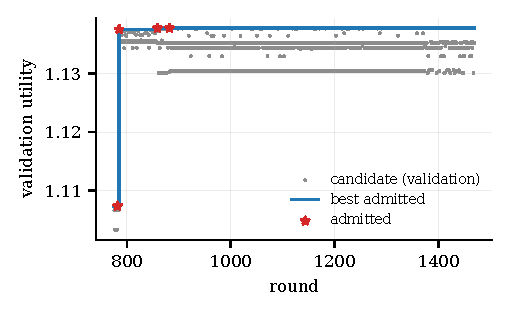
\includegraphics[width=\linewidth]{figures/fig_fw_validation.pdf}
  \caption{\textbf{Validation utility has plateaued.} Grey: each round's
  candidate adapter on the validation families. Blue: best admitted model.
  Stars: the four admitted candidates (rounds 775--1469).}
  \label{fig:fw-validation}
\end{figure}

\begin{figure}[t]
  \centering
  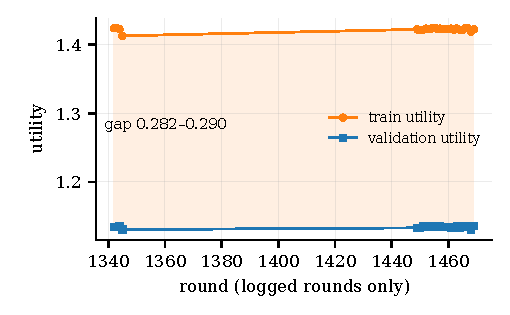
\includegraphics[width=\linewidth]{figures/fig_fw_train_val.pdf}
  \caption{\textbf{Train and validation utility, with the gap shown.} Only
  rounds whose full summaries are retained are plotted (25 rounds between
  1342 and 1469); the line joins non-consecutive rounds across the gap.}
  \label{fig:fw-trainval}
\end{figure}

\begin{figure*}[t]
  \centering
  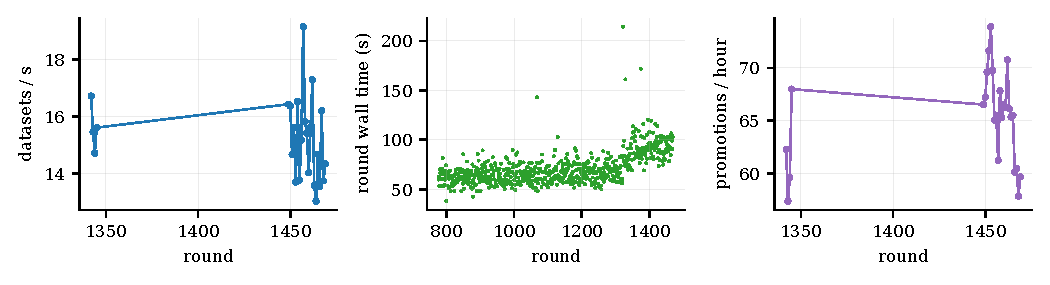
\includegraphics[width=\linewidth]{figures/fig_fw_telemetry.pdf}
  \caption{\textbf{Loop telemetry.} Left: datasets evaluated per second.
  Middle: wall time between consecutive rounds. Right: programs promoted into
  the pools per hour. The run directory occupied 290\,MB at the snapshot.}
  \label{fig:fw-telemetry}
\end{figure*}

